\documentclass[11pt,a4paper]{article}
\usepackage[margin=25mm]{geometry}
\usepackage{fontspec,unicode-math,amsmath,booktabs,graphicx,hyperref}
\setmainfont{STIXGeneral}\setmathfont{STIX Two Math}
\setlength{\parindent}{0pt}\setlength{\parskip}{6pt}\setlength{\emergencystretch}{2em}
\hypersetup{hidelinks}
\title{Coset geometries and symmetric group markings}
\author{Six-original manuscript comparison}\date{}
\begin{document}\maketitle
The six complete original representations contain 144,877 characters. Both complete common papers and all six applications contain 149,071. The fixed primary comparison is
\[
 R=\frac{\sum_{i=1}^6c(S_i)}{c(U_B)+c(U_{B6})+\sum_{i=1}^6c(B_i)}
 =\frac{144877}{44905+29398+74768}
 =\mathbf{0.971866}.
\]
\textbf{This is whole-topic expansion, not achieved whole-topic compression.}
The replacement is 4,194 characters longer in this coordinate. The primary counts raw, untrimmed NFC characters excluding whitespace; it was fixed before calculation and retains the previous B convention. No metric or boundary was changed to obtain a preferred result.

The entire sixteen-page prior common paper and ten-page supplement are paid once each, with all thirty application pages. The two-page archived finite-neighbor precursor is already incorporated in the supplement and is not charged again. No old common passage is removed because it is no longer on a particular logical route.

The source side contains five full PDFs and N001's complete literal authored rendering. N001's original PDF remains unavailable, so this is not an all-PDF comparison. The L040 identification cover remains in the primary source. Titles, abstracts, whole tables, proofs, references and extractable figure labels stay counted.

\textbf{Conditional on prior acquisition.} Each factor below is $c(S_i)/c(B_i)$ after acquiring \emph{both whole common papers and the complete required topic premises}. These are complete local applications; no sibling application is silently assumed.
\begin{center}\begin{tabular}{llrrr}\toprule
Original & App & Source & Application & Conditional\\\midrule
N001 & B1 & 14,519 & 7,371 & 1.969746\\
N003 & B2 & 17,780 & 9,155 & 1.942108\\
N008 & B3 & 18,009 & 11,132 & 1.617769\\
L030 & B4 & 22,704 & 12,286 & 1.847957\\
L040 & B5 & 51,894 & 29,321 & 1.769858\\
L047 & B6 & 19,971 & 5,503 & 3.629111\\
\bottomrule\end{tabular}\end{center}
All five earlier conditional fraction records are exactly unchanged in all thirty coordinates. L047 adds 19,971 source characters, 29,398 common characters and 5,503 application characters. The prior whole factor 1.094035 and the current 0.971866 describe different complete editions; conditional savings do not cancel the added common cost.
\newpage
\begin{center}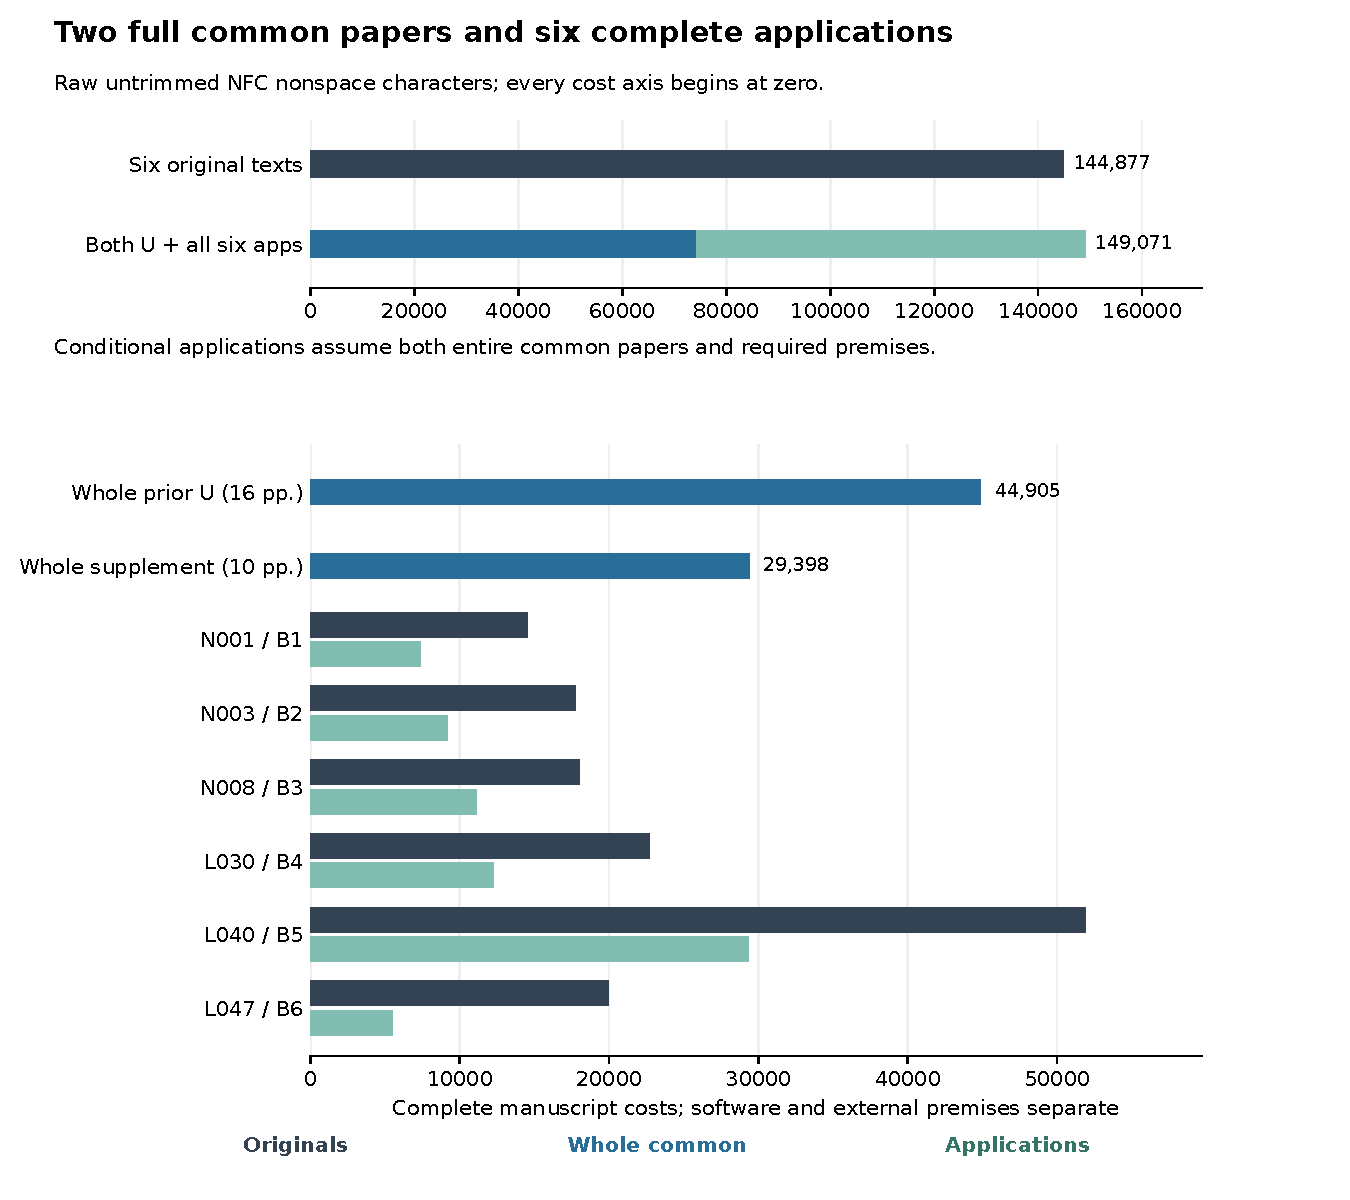
\includegraphics[width=\linewidth]{costs.pdf}\end{center}
The upper bars compare all six originals with both common papers and every application. The lower bars show the same whole common acquisition and each complete source/application pair. All 23 colored rectangles represent actual manuscript costs, not ratios or proof-node counts. Each axis starts at zero.

Executable software is excluded symmetrically from source and replacement manuscript costs. This includes required computations: their proof role is unchanged, although their implementation costs lie outside this scalar. Mathematical algorithm and proof prose remain counted. Unknown historical software prevents a software-inclusive factor.
\newpage
\begin{center}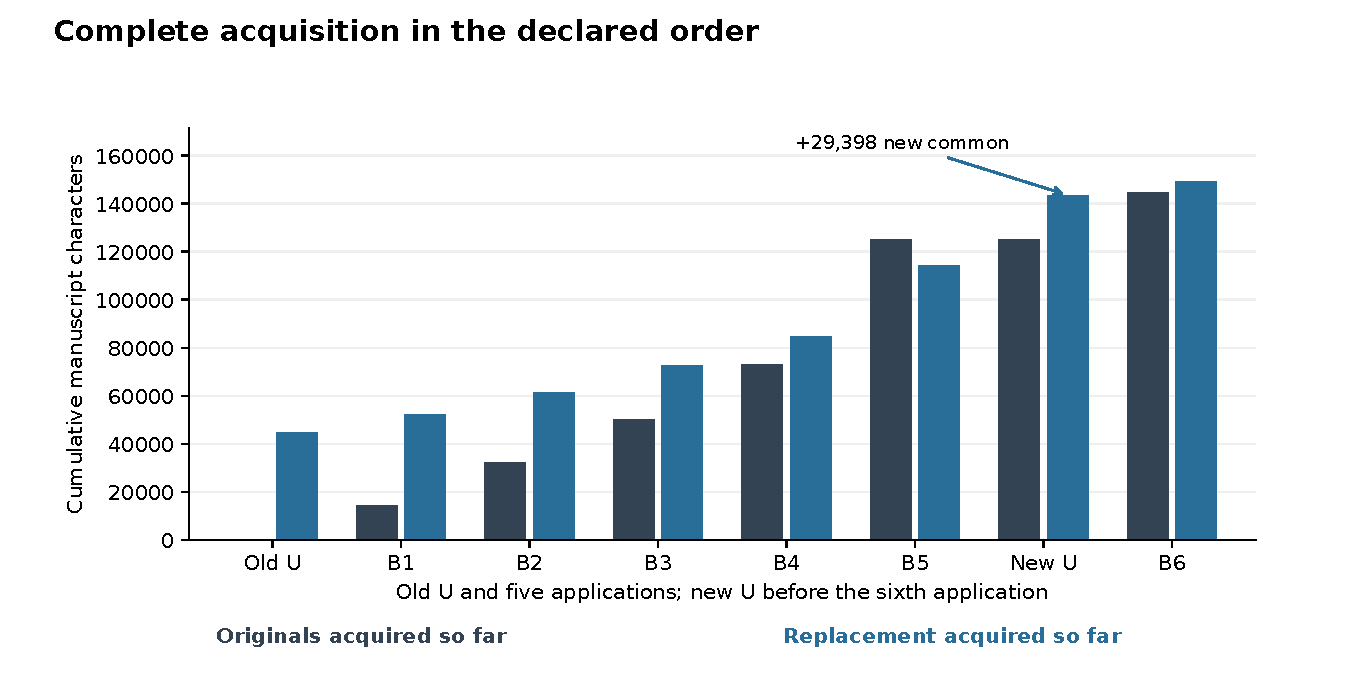
\includegraphics[width=\linewidth]{cumulative.pdf}\end{center}
Stage zero acquires the entire old common paper (44,905 characters), followed by the five earlier complete source/application pairs. A separate stage then acquires the whole new supplement (29,398 characters): this is the visible common-theory cost jump before B6. The final stage adds L047 and its complete application. Both common papers total 74,303 characters. These eight stages show an explicit acquisition order, with no optimality or predetermined sawtooth claim. The conditional table on page 1 assumes both common papers and all required topic premises have already been acquired.

\textbf{Whole-file inventory, separate from the manuscript factor.}
\begin{center}\small\begin{tabular}{lrrr}\toprule
Role & Files & NFC nonspace & Literal bytes\\\midrule
Required / auxiliary programs & 8 & 22,455 & 24,859\\
Optional validation & 2 & 5,440 & 6,537\\
Operational drivers & 5 & 30,987 & 34,448\\
Partial formal files & 2 & 8,377 & 11,726\\
\bottomrule\end{tabular}\end{center}
The ten mathematical files comprise eight required or auxiliary premises and two optional validations. The latter are not required acquisition. The six added required files include \path{retained/finite_boundary/run.g}: it fixes the exact roster and is not merely a driver. The source names Magma and PrimitiveGroupSims; our required implementations use GAP.

The two complete seven-page code appendices cost 13,170 and 16,472 characters, 29,642 together. Their ten complete raw alternatives cost 27,895 characters and 31,396 literal bytes. Printed and raw are alternatives, never additive copies. Neither is used for an asymmetric software-inclusive factor. The five operational drivers and two Lean modules stay separate; fourteen inherited declarations remain partial evidence. Four archived independent-review tools are bound as provenance, not added proof premises. GAP algorithms and group catalogues retain unknown external costs.
\newpage
\textbf{Sensitivity of the complete written comparison.}
\begin{center}\small\begin{tabular}{lrrr}\toprule
Unit & Raw complete & Raw selected & Calibrated\\\midrule
NFC: Whitespace tokens & 1.025682 & 1.012677 & 1.012677\\
NFC: Alphanumeric units & 1.105842 & 1.092779 & 1.093481\\
NFC: Nonspace characters & 0.971866 & 0.957008 & 0.957008\\
NFC: Collapsed-space characters & 0.981464 & 0.966926 & 0.966926\\
NFC: Collapsed UTF-8 bytes & 0.939616 & 0.926135 & 0.926108\\
NFKC: Whitespace tokens & 1.027724 & 1.014723 & 1.014723\\
NFKC: Alphanumeric units & 1.105842 & 1.092779 & 1.093481\\
NFKC: Nonspace characters & 0.973808 & 0.958954 & 0.958954\\
NFKC: Collapsed-space characters & 0.983424 & 0.968888 & 0.968888\\
NFKC: Collapsed UTF-8 bytes & 0.998361 & 0.984058 & 0.982731\\
\bottomrule\end{tabular}\end{center}
The complete record contains thirty settings, with 210 main exact fractions: one whole-topic and six conditional comparisons per setting. Sixty additional fractions give the whole-topic and L040 conditional article-only sensitivities. Exact unreduced costs, reduced fractions and forty-two significant-digit decimal strings are provided. Six-place reader rounding uses exact decimal division.

\textbf{L040 article-only sensitivity.} Removing only its accepted identification-cover text changes the primary source total to 144,096, leaving every replacement cost unchanged. The whole factor is 0.966627 and L040's conditional is 1.743222. The other five conditionals are unchanged. The primary continues to include the cover.

All 480 accepted main document cells (450 PDF and 30 literal-rendering cells), thirty article-only cells and 170 whole-file cells remain unchanged. There are fifteen measured PDFs over 134 physical pages, including the separate fourteen program pages, plus the literal N001 rendering. The new L047 source is twelve pages and its local application three. Raw selected and calibrated coordinates reuse the accepted exact furniture exclusions and occurrence-bound repairs; none is reevaluated here.

\textbf{Scientific scope.} The accepted corrected principal contracts and retained inputs remain the authority. L047's 58 dispositions are not 58 originals. Its 23 finer ancillary Table 3 reports remain outside the regenerated scope while their whole source text is charged. The source's Conjecture 1.1 was already resolved in L044; this comparison adds no question answer. Earlier source corrections and exclusions remain explicit in their source maps.

Full graphics and layout, unavailable external proofs, catalogue construction, historical software and complete formalization have unknown costs, not zero. These are manuscript comparisons for the declared principal outputs, not claims that every source passage or all software has been replaced. No source, proof, question or formal credit follows from a factor.

The numerical author is enumeration\_volume. The new input author is rewrite\_termination, with distinct root input review/adoption; enumeration\_review authored the new L047 science. Earlier B authorship and the numerical author's distinct review of the root finite-neighbor lemma are disclosed in the packet. This calculation reuses adopted inputs and earlier reader mechanics; it reruns no source extraction, mathematical census or Lean proof.
\end{document}
